% Chapter 2

\chapter{Continuations en aplicaciones web}
% Write in your own chapter title
\label{Capitulo 2}
\lhead{Capítulo 2. \emph{Continuations en aplicaciones web}} % Write in your own chapter title to set the page header

%-->
% Explicación teórica (no matematica, ni con scheme) de first-class continuations
% Modificaciones/extensiones a continuations
% Aplicaciones web
%- Inconvenientes cuando falta continuations (con MVC)
%	- Flujo de control
%	- Estado
%- Component como bloque de contrucción
%	- Backtracking
%	- Transacciones
%- Combinación con las nuevas tecnologías
%	- AJAX
%	- Server Push
%-->

%Una de las implementaciones más sencillas de \emph{first-class continuations} es la mencionada por \emph{Hieb et al.}\cite[p.~2]{Hieb90}. Ésta consiste en reemplazar la \emph{pila de llamadas tradicional} por una lista enlazada de registros de activación (ver Figura \ref{ContinuationsActivationRecords}).

%\begin{figure}[ht!]
%\centering
%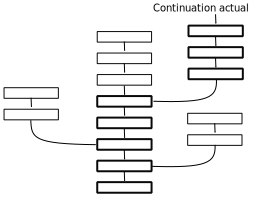
\includegraphics[scale=1]{ContinuationsActivationRecords}
%\caption{Implementación de continuations a partir de una lista enlazada de registros de activación}
%\label{ContinuationsActivationRecords}
%\end{figure}

%En este modelo los registros de activación previamente creados nunca se sobrescriben, y en cambio se crea un nuevo registro por cada llamada. Como contraparte, el adminis\-trador del almacenamiento eliminará un registro en desuso cuando éste ya no pueda ser alcanzado por una \emph{continuation}.

%Existen variantes para esta implementación en las que se desarrollan distintas estructuras de control como \emph{loops}, \emph{nonblind backtracking}\cite{Sussman98}, co-rutinas\cite{Haynes86,Hieb90a,Hieb94}, y engines\cite{Haynes87,Dybvig88} que escapan al alcance de esta tesis.

Como se mencionó en el capítulo anterior, el objetivo de esta tesis es incorporar la información brindada por los sensores de un dispositivo tecnológico en un framework de aplicaciones web basado en continuations.

A partir de esto, es importante destacar que las aplicaciones web desarrolladas con continuations comienzan a surgir en el año 1995. Y gran parte del aporte lo realizaron \emph{Ladd et al.}\cite{Ladd95} y \emph{Quiennec} \cite{Queinnec01}, quienes fueron los primeros en proponer esta variante con el fin de sobrellevar la falta de estado del protocolo \emph{HTTP}\footnote{Del inglés ``Hypertext Transfer Protocol''.}.

% verificar si no queda mejor dado vuelta...

%\emph{Ladd et al.}\cite{Ladd95} y \emph{Quiennec} \cite{Queinnec01} son los primeros en proponer una variante de continuations en el marco de las \emph{aplicaciones web}, para solucionar la falta de estado del protocolo \emph{HTTP}\footnote{Del inglés ``Hypertext Transfer Protocol''.}.

Luego, en el 2004, \emph{Ducasse et al.}\cite{Ducasse04} explica las ventajas de utilizar cierta implementación de continuations para aplicaciones web con respecto a otros frameworks alternativos.

%A continuación se enumeran los \emph{inconvenientes de desarrollar una aplicación web sin continuations}. Luego, se presenta una solución basada en \emph{componentes} reutilizables, que es como Seaside\footnote{Framework para desarrollar aplicaciones web orientado a objetos basado en continuations. Ver \url{http://www.seaside.st/}.} se encuentra implementado actualmente. Por último se describe cómo pueden ser combinadas nuevas tecnologías, como \emph{AJAX}\footnote{Del inglés ``Asynchronous Javascript And XML''.} y \emph{Server Push}\footnote{Técnica que permite enviar información desde el Servidor hacia el Cliente, sin que este último la haya solicitado explícita\-mente.}, con un framework de las características de Seaside.

A continuación se enumeran los \emph{inconvenientes de desarrollar una aplicación web sin continuations}. Luego, como contraparte se presenta Seaside\footnote{Framework para desarrollar aplicaciones web orientado a objetos basado en continuations. Ver \url{http://www.seaside.st/}.}, una solución basada en continuations a partir de \emph{componentes} reutilizables, ampliamente utilizada por los desarrolladores de aplicaciones web.

%Por último, dado que Seaside va a ser el framework en donde se realizarán las pruebas pertinentes, se describirá como ha sido extendido para soportar funcionalidades como \emph{AJAX}\footnote{Del inglés ``Asynchronous Javascript And XML''.} y \emph{Server Push}\footnote{Técnica que permite enviar información desde el Servidor hacia el Cliente, sin que este último la haya solicitado explícita\-mente.}, que son técnicas utilizadas en gran parte de las aplicaciones web de la actualidad.
Por último, y considerando que Seaside va a ser el framework en donde se realizarán las pruebas pertinentes, se describirá como ha sido extendido para soportar funcionalidades como \emph{AJAX}\footnote{Del inglés ``Asynchronous Javascript And XML''.} y \emph{Server Push}\footnote{Técnica que permite enviar información desde el Servidor hacia el Cliente, sin que este último la haya solicitado explícita\-mente.}, que son técnicas utilizadas en gran parte de las aplicaciones web de la actualidad.


\section{Inconvenientes de los frameworks sin continuations}

Al desarrollar aplicaciones web con frameworks que no se basan en continuations existen un conjunto de inconvenientes y/o contratiempos que deben ser resueltos. Algunos de ellos consecuencia de una escasa abstracción sobre el protocolo HTTP, y otros por restricciones planteadas por el esquema REST\cite[p.~76]{Fielding00} existente en muchos frameworks.

%Como sintetiza \emph{Ducasse et al.}\cite[p.~234]{Ducasse04} existen dos tipos de dificultades cuando se utilizan la mayoría de los frameworks actuales (tales como Struts\footnote{\url{http://struts.apache.org/}}, Symfony\footnote{\url{http://www.symfony-project.org/}}, ASP.net\footnote{\url{http://www.asp.net/}}, Rails\footnote{\url{http://rubyonrails.org/}}, etc.): los relacionados con la lógica del \emph{flujo de control} y los que conciernen al \emph{estado} entre las interacciones del usuario.

Como sintetiza \emph{Ducasse et al.}\cite[p.~234]{Ducasse04} existen dos tipos de dificultades cuando se utiliza algún framework alternativo (tal como Servlets/JSP\footnote{\url{http://java.sun.com/products/servlet/} y \url{http://java.sun.com/products/jsp/}}, PHP\footnote{\url{http://www.php.net/}}, ASP\footnote{\url{http://msdn.microsoft.com/en-us/library/ms972347.aspx}}, JSP\footnote{\url{http://java.sun.com/products/jsp/}} o Zope\footnote{\url{http://www.zope.org}}): los relacionados con la lógica del \emph{flujo de control} y los que conciernen al \emph{estado} entre las interacciones del usuario.


\subsection{Flujo de control}

Al considerar el flujo de control de estos últimos frameworks, se observa que fallan en proporcionar una abstracción de alto nivel para especificar cómo son enlazadas las páginas.

La lógica del flujo de control debería estar implementada idealmente en una única porción de código, que utilice estructuras de control comunes al lenguaje de programación utilizado para especificar el modelo de negocios. Desafortunadamente, esta forma de programar es opuesta a lo que el protocolo HTTP establece (con sus mensajes de solicitud y respuesta).

Los problemas más relevantes relacionados con el flujo de control son:

\begin{description}

\item[Mezclar la lógica de aplicación con la lógica de los componentes.]

La interacción del usuario en una aplicación web puede ser vista como dos tareas que se repiten en el tiempo: la primera es \emph{generar la página} y la segunda \emph{procesar los datos} cuando el usuario los envíe. Estas tareas se ejecutan de forma separada y levemente conectadas.

De esta forma, la decisión de \emph{``¿qué es lo que hago a continuación?''} está asociada a la parte de procesamiento de datos de la última página, en lugar de ser definido como un \emph{flujo de control} a más alto nivel.

En los frameworks orientados a páginas cada componente debe indicar como interactúa con el resto. Así, cada página en una secuencia tendrá un enlace \emph{estructurado de forma estática}\footnote{Traducción no literal de ``hardcoded''.} a la próxima.

\item[Incapacidad para componer flujos de control.]

No todos los frameworks para desarrollar aplicaciones web proveen la capacidad de reutilizar componentes (en donde cada uno posee su propio flujo de control). Esto dificulta la posibilidad de trabajar con \emph{múltiples flujos de control} en una misma página.

\item[Controlar el flujo del programa.]

Dado que el usuario puede clonar una página e ir hacia atrás en el historial, es necesario contar con la posibilidad de \emph{invalidar} un flujo de control luego de que una \emph{transacción} se haya concluido y aceptado.

\end{description}


\subsection{Estado}
\label{ControlFlowStates}

Por otra parte, una aplicación web típica tiene que tratar con tres tipos de estados: el asociado a la \emph{interfaz gráfica con el usuario} (de cada componente), el del \emph{modelo del dominio} (relacionado con las instancias del modelo del negocio) y el referido a la \emph{sesión de usuario} (se encarga de mantener estados globales de la sesión, que no pertenecen al modelo de negocios ni a la interfaz gráfica con el usuario). Un ejemplo de este ultimo tipo de estado es la identificación del usuario, que suele ser común a todos los componentes.

Pero administrar el estado en el ámbito de una aplicación cliente-servidor es complejo como consecuencia del flujo de control no lineal. Esto, principalmente, es causado por la incapacidad del protocolo HTTP de mantener estados y por las capacidades de los navegadores web (clonar y/o retroceder).

Actualmente, en los frameworks orientados a páginas el estado es codificado en las respuestas al cliente. Esta solución temporal conduce a los siguientes inconvenientes:


\begin{description}

\item[Codificar el estado.]

Cuando el estado del modelo del dominio debe ser tenido en cuenta sobre una secuencia de páginas, cada página tiene que pasar la información recibida desde las páginas anteriores y trasladarla a la próxima. Esto produce que el código no sea reutilizable por su dependencia de las páginas precedentes.

\item[Colisión de los nombres.]

Puede haber colisiones en los nombres de las \emph{URL}\footnote{Del inglés ``Uniform Resource Locator''.} o en los campos de los formularios. El programador debe encargarse de que los identificadores sean únicos a lo largo de una página. Esto se vuelve especialmente un problema cuando se desean reutilizar los componentes.

\item[Mezclar la lógica de presentación con la del dominio.]

Para codificar el estado en una página se deberá mezclar la generación de HTML\footnote{Del inglés ``Hypertext Markup Language''.} con la lógica de dominio usando \emph{templates} o la concatenación de \emph{strings}. Esto terminará produciendo código fuente difícil de leer.

\end{description}


\section{El \emph{Componente} como bloque de construcción}

A partir de los inconvenientes planteados con el flujo de control y la administración de estados, existen frameworks como Seaside en los que se propone la construcción de una página a partir de \emph{componentes}\footnote{Seaside lo implementa en la clase \emph{WAComponent}.}. Cada componente se encarga de definir la interfaz de usuario y el flujo de control de una parte de la aplicación. A diferencia de los frameworks orientados a páginas la instancia de un componente a menudo perdura a lo largo de la sesión del usuario.

En cada solicitud el framework le permite a cada componente evaluar sus \emph{callbacks} y \emph{renderizar} su estado actual en un \emph{stream de respuesta}.

Las características más importantes de esta aproximación son: el \emph{renderizado}, la \emph{composición de componentes} y los \emph{action callbacks}.

\begin{description}

\item[Renderizado.]

Cada componente que es visible en una aplicación web tiene un \emph{método de enganche}\footnote{Del inglés ``callback''.}, que permite definir su aspecto visual. Este método es llamado con un \emph{stream de respuesta} como parámetro, permitiendo especificar las características gráficas y de comportamiento de cada componente con el mismo lenguaje en el cual está implementado el modelo de negocios.

\item[Composición de componentes.]

Para la construcción de una aplicación web un componente puede contener a muchos otros. De esta forma una ``página'' sería definida como un componente compuesto. Por otra parte existe un componente específico denominado \emph{Task}, que se encarga solamente de definir un flujo de control, y así prescindir del \emph{renderizado}.

\item[Action Callbacks.]

Los componentes pueden reaccionar a las acciones realizadas por el usuario a través de los \emph{action callbacks}. Estos son definidos sobre los \emph{botones}, \emph{enlaces} y por cada campo de un formulario mediante la utilización de un \emph{bloque de código o functor} al momento de describir el comportamiento de un componente.

El \emph{action callback} de un campo del formulario contiene un argumento que representará al valor del campo en cuestión. Mientras que para los enlaces y botones el bloque no contiene ningún argumento, en estos se define el flujo de control del componente o de la aplicación.

\end{description}

Dado que cada componente define su propio flujo de control independiente de los otros mostrados en la misma página, un componente o aplicación puede tener múltiples flujos de control.

Cada vez que el usuario utilice un \emph{enlace} o un \emph{botón} en un componente realizará un paso hacia adelante en su flujo de control, mientras el resto de los flujos de control permanecen en el mismo estado.

Para facilitar la creación y administración de múltiples flujos de control los frameworks basados en \emph{componentes} proporcionan los métodos \textbf{call:} y \textbf{answer:}.

\begin{description}

\item[Call.]

Mediante este método un componente (por ejemplo \emph{A}) puede pasarle el control a cualquier otro componente (en este caso \emph{B}). Durante este tiempo el componente original (\emph{A}) es temporalmente reemplazado por el otro componente (\emph{B}). Esto es posible mediante el envío del mensaje \textbf{call:} al componente \emph{A} y enviándole como parámetro el componente \emph{B}.

\item[Answer.]

Mediante este método un componente (por ejemplo el \emph{B}) puede devolver el control a aquel componente desde el cual ha sido llamado (en este caso el \emph{A}). Cada componente eventualmente devolverá el control de la ejecución en algún punto, e inclusive puede retornar un objeto que modele la respuesta. Esto es posible mediante el envío del mensaje \emph{answer:} al componente \emph{B} y enviándole como parámetro el objeto que modela la respuesta.

\end{description}

Aunque desde la perspectiva del desarrollador el código es lineal, existen algunas cuestiones relacionadas con el estado de la aplicación web que deben ser explicadas.

Seaside permite la \emph{clonación} de una página y \emph{volver} al estado anterior. De esta forma es necesario que exista cierto mecanismo que se encargue de mantener el estado de la \emph{interfaz gráfica} y del \emph{modelo del dominio}, ambos mencionados en la sección \nameref{ControlFlowStates} (\ref{ControlFlowStates}).


\subsection{Backtracking}

Dado que cada componente tiene su propio estado, el cual es guardado en las variables de instancia (por ejemplo un componente que muestra un listado de elementos de forma paginada recordará el numero de la página actual). Cuando el usuario \emph{vuelve} hacia atrás con el navegador web, las variables de instancia del componente pueden no representar el estado que el usuario visualiza.

Una forma de mantener el estado de los componentes en sincronía con lo que visualiza el navegador web es mediante la utilización de continuations. Para esto, Seaside ofrece un mecanismo para seleccionar qué variables de instancia deben ser \emph{rastreadas}\footnote{Del inglés ``backtracking''.}. Después de cada respuesta enviada al cliente, el framework guarda una copia exacta de los objetos seleccionados mediante la creación de un \emph{registro de activación}.

La sesión del usuario almacena el registro como una variable temporal dentro del proceso que envía la \emph{respuesta} al cliente y que luego recibirá la próxima \emph{solicitud}. El registro se vuelve persistente hasta un momento en el futuro en el cual el flujo de control requiera retomar la ejecución de este componente almacenado.

Al momento de restablecer el \emph{contexto de ejecución} y antes de procesar la solicitud del cliente, el registro restablece los objetos registrados y la \emph{continuation} es procesada.

Esto asegura que cuando se procesa una solicitud, los valores son los mismos que cuando la respuesta previa fue creada.


\subsection{Transacciones}

En ciertas aplicaciones complejas suele ser necesario interceder para prevenir que el usuario retroceda a la página anterior. Seaside implementa el método ``\emph{isolate: aBlockClosure}'' para controlar el flujo de control. Este método recibe un \emph{bloque de código} o \emph{functor} como argumento, el cual es tratado como una transacción.

La transacción le garantiza al usuario poder ir hacia adelante y hacia atrás, siempre y cuando permanezca dentro del \emph{bloque transaccional}. Sin embargo, una vez terminada la transacción el usuario no podrá volver hacia atrás, dado que la transacción ha sido dada por concluida.


\section{Combinación con las nuevas tecnologías}

Al considerar el requisito de extender una aplicación web basada en continuations, es necesario corroborar como se han realizado otras extensiones al framework presentado.

Para esto, a continuación se repasará como otras librerías de terceros han incorporado dos protocolo de comunicación como \emph{AJAX}\footnote{Es la sigla de ``Asynchronous Javascript And XML''.} y \emph{Server Push} al framework Seaside.


\subsection{Asynchronous Javascript And XML}

El uso masivo de las aplicaciones web comienza a evidenciar que las interacciones del usuario se realizan sobre ciertas partes de una página, mientras que otras partes permanecen inalteradas.

Como consecuencia se comienza a trabajar en una abstracción que permita desacoplar la interacción del usuario de la carga de la página, con el fin que puedan realizarse solicitudes de forma asíncronas y manipular las respuestas para que puedan ser incluidas en la porción de página que debe ser actualizada.

Esta abstracción es denominada \emph{AJAX} y es totalmente compatible con el protocolo HTTP, dado que mantiene el requisito que una \emph{respuesta} del servidor solo será dada a partir de una \emph{solicitud} del cliente\footnote{Detallado en la \emph{RFC2616} (\url{http://www.ietf.org/rfc/rfc2616.txt}).}.

% Se denomina \emph{AJAX} a la abstracción que brinda la posibilidad de que el navegador web realice solicitudes de forma asíncronas al servidor, sin la necesidad de recargar toda la página. Así, la información recibida es utilizada para actualizar sólo una porción de la página. Esta técnica es totalmente compatible con el protocolo HTTP, dado que mantiene el ciclo de solicitud/respuesta\footnote{Detallado en la \emph{RFC2616} (\url{http://www.ietf.org/rfc/rfc2616.txt}).}.

Para soportar \emph{AJAX} de una forma transparente al desarrollador, Seaside agrega la clase \emph{SUComponent} que es una especialización del \emph{WAComponent}\footnote{Componente base del framework Seaside.} (ver Figura \ref{SUComponent}).

\begin{figure}[ht!]
\centering
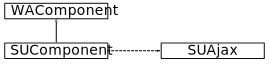
\includegraphics[scale=1]{SUComponent}
\caption{Extensión de Seaside para soportar AJAX}
\label{SUComponent}
\end{figure}

El componente \emph{SUComponent} es una implementación del patrón \emph{Abstract Factory}\cite{Gamma95} que permite la creación de objetos \emph{SUAjax}.

Cada instancia de \emph{SUAjax} representa una posible solicitud asíncrona que puede realizar el cliente. Luego, en el momento del \emph{renderizado}, el framework podrá procesar la respuesta que posteriormente será enviada al cliente.


\subsection{Server Push}

La utilización de AJAX dio lugar a un nuevo conjunto de aplicaciones web que mejoran la interacción e intercomunicación entre distintos usuarios.

Para esto un navegador web debe preguntar al servidor de forma periódica si existen actualizaciones para cierto usuario. Cuanto mas seguido pregunta, más interactiva se vuelve la aplicación. Aunque existen ciertas aplicaciones web en donde el cliente consulta muchas veces y las actualizaciones son por momentos pocas y por momentos muchas.

Esto planteó otra situación, y es que los navegadores solo pueden obtener las actualizaciones de los otros usuarios a partir de solicitarlas al servidor, como consecuencia del ciclo solicitud/respuesta del protocolo HTTP.

Para mejorar esto, \emph{Server Push} utiliza conexiones \emph{HTTP} de larga duración para reducir la \emph{latencia} de comunicación entre el \emph{servidor web} y el \emph{navegador}. Esto implica una \emph{optimización} con respecto a AJAX, al permitir que un servidor inyecte información en un cliente en particular.

Desde el punto de vista del cliente, en lugar de solicitar reiteradamente al servidor por la existencia de alguna actualización, el navegador deja una conexión abierta\footnote{Conceptualmente se considera que es una conexión abierta, aunque en realidad se suele utilizar un \emph{timeout} elevado que eventualmente podrá cerrar la conexión.}. De esta forma el servidor cuenta siempre con un canal para enviar información, teniendo la capacidad de establecer el momento en el que el cliente recibirá la información.

Para implementar \emph{Server Push}, \emph{Seaside} agrega la clase \emph{Meteoroid} que es una especiali\-zación del \emph{WAComponent} (ver Figura \ref{Meteoroid}).

\begin{figure}[ht!]
\centering
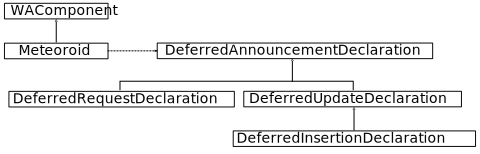
\includegraphics[scale=1]{Meteoroid}
\caption{Extensión de Seaside para soportar Server Push}
\label{Meteoroid}
\end{figure}

El componente \emph{Meteoroid} permite actualizar el contenido del cliente web mediante tres acciones: una \emph{solicitud}, la \emph{inserción} y la \emph{actualización}.

La \emph{solicitud} posibilita que el servidor obligue al cliente a realizar una \emph{solicitud asíncrona mediante AJAX}.

Por otra parte, mientras la \emph{inserción} siempre agrega el contenido al final de una \emph{etiqueta HTML}, la \emph{actualización} reemplaza el contenido completo.